% Options for packages loaded elsewhere
\PassOptionsToPackage{unicode}{hyperref}
\PassOptionsToPackage{hyphens}{url}
\PassOptionsToPackage{dvipsnames,svgnames,x11names}{xcolor}
%
\documentclass[
  letterpaper,
  DIV=11,
  numbers=noendperiod]{scrartcl}

\usepackage{amsmath,amssymb}
\usepackage{iftex}
\ifPDFTeX
  \usepackage[T1]{fontenc}
  \usepackage[utf8]{inputenc}
  \usepackage{textcomp} % provide euro and other symbols
\else % if luatex or xetex
  \usepackage{unicode-math}
  \defaultfontfeatures{Scale=MatchLowercase}
  \defaultfontfeatures[\rmfamily]{Ligatures=TeX,Scale=1}
\fi
\usepackage{lmodern}
\ifPDFTeX\else  
    % xetex/luatex font selection
\fi
% Use upquote if available, for straight quotes in verbatim environments
\IfFileExists{upquote.sty}{\usepackage{upquote}}{}
\IfFileExists{microtype.sty}{% use microtype if available
  \usepackage[]{microtype}
  \UseMicrotypeSet[protrusion]{basicmath} % disable protrusion for tt fonts
}{}
\makeatletter
\@ifundefined{KOMAClassName}{% if non-KOMA class
  \IfFileExists{parskip.sty}{%
    \usepackage{parskip}
  }{% else
    \setlength{\parindent}{0pt}
    \setlength{\parskip}{6pt plus 2pt minus 1pt}}
}{% if KOMA class
  \KOMAoptions{parskip=half}}
\makeatother
\usepackage{xcolor}
\setlength{\emergencystretch}{3em} % prevent overfull lines
\setcounter{secnumdepth}{-\maxdimen} % remove section numbering
% Make \paragraph and \subparagraph free-standing
\makeatletter
\ifx\paragraph\undefined\else
  \let\oldparagraph\paragraph
  \renewcommand{\paragraph}{
    \@ifstar
      \xxxParagraphStar
      \xxxParagraphNoStar
  }
  \newcommand{\xxxParagraphStar}[1]{\oldparagraph*{#1}\mbox{}}
  \newcommand{\xxxParagraphNoStar}[1]{\oldparagraph{#1}\mbox{}}
\fi
\ifx\subparagraph\undefined\else
  \let\oldsubparagraph\subparagraph
  \renewcommand{\subparagraph}{
    \@ifstar
      \xxxSubParagraphStar
      \xxxSubParagraphNoStar
  }
  \newcommand{\xxxSubParagraphStar}[1]{\oldsubparagraph*{#1}\mbox{}}
  \newcommand{\xxxSubParagraphNoStar}[1]{\oldsubparagraph{#1}\mbox{}}
\fi
\makeatother


\providecommand{\tightlist}{%
  \setlength{\itemsep}{0pt}\setlength{\parskip}{0pt}}\usepackage{longtable,booktabs,array}
\usepackage{calc} % for calculating minipage widths
% Correct order of tables after \paragraph or \subparagraph
\usepackage{etoolbox}
\makeatletter
\patchcmd\longtable{\par}{\if@noskipsec\mbox{}\fi\par}{}{}
\makeatother
% Allow footnotes in longtable head/foot
\IfFileExists{footnotehyper.sty}{\usepackage{footnotehyper}}{\usepackage{footnote}}
\makesavenoteenv{longtable}
\usepackage{graphicx}
\makeatletter
\def\maxwidth{\ifdim\Gin@nat@width>\linewidth\linewidth\else\Gin@nat@width\fi}
\def\maxheight{\ifdim\Gin@nat@height>\textheight\textheight\else\Gin@nat@height\fi}
\makeatother
% Scale images if necessary, so that they will not overflow the page
% margins by default, and it is still possible to overwrite the defaults
% using explicit options in \includegraphics[width, height, ...]{}
\setkeys{Gin}{width=\maxwidth,height=\maxheight,keepaspectratio}
% Set default figure placement to htbp
\makeatletter
\def\fps@figure{htbp}
\makeatother

\usepackage{booktabs}
\usepackage{caption}
\usepackage{longtable}
\usepackage{colortbl}
\usepackage{array}
\usepackage{anyfontsize}
\usepackage{multirow}
\KOMAoption{captions}{tableheading}
\makeatletter
\@ifpackageloaded{caption}{}{\usepackage{caption}}
\AtBeginDocument{%
\ifdefined\contentsname
  \renewcommand*\contentsname{Table of contents}
\else
  \newcommand\contentsname{Table of contents}
\fi
\ifdefined\listfigurename
  \renewcommand*\listfigurename{List of Figures}
\else
  \newcommand\listfigurename{List of Figures}
\fi
\ifdefined\listtablename
  \renewcommand*\listtablename{List of Tables}
\else
  \newcommand\listtablename{List of Tables}
\fi
\ifdefined\figurename
  \renewcommand*\figurename{Figure}
\else
  \newcommand\figurename{Figure}
\fi
\ifdefined\tablename
  \renewcommand*\tablename{Table}
\else
  \newcommand\tablename{Table}
\fi
}
\@ifpackageloaded{float}{}{\usepackage{float}}
\floatstyle{ruled}
\@ifundefined{c@chapter}{\newfloat{codelisting}{h}{lop}}{\newfloat{codelisting}{h}{lop}[chapter]}
\floatname{codelisting}{Listing}
\newcommand*\listoflistings{\listof{codelisting}{List of Listings}}
\makeatother
\makeatletter
\makeatother
\makeatletter
\@ifpackageloaded{caption}{}{\usepackage{caption}}
\@ifpackageloaded{subcaption}{}{\usepackage{subcaption}}
\makeatother

\ifLuaTeX
  \usepackage{selnolig}  % disable illegal ligatures
\fi
\usepackage{bookmark}

\IfFileExists{xurl.sty}{\usepackage{xurl}}{} % add URL line breaks if available
\urlstyle{same} % disable monospaced font for URLs
\hypersetup{
  pdftitle={Group 14: Measles susceptibility in Edinburgh},
  colorlinks=true,
  linkcolor={blue},
  filecolor={Maroon},
  citecolor={Blue},
  urlcolor={Blue},
  pdfcreator={LaTeX via pandoc}}


\title{Group 14: Measles susceptibility in Edinburgh}
\author{}
\date{}

\begin{document}
\maketitle


\section{Introduction}\label{introduction}

Measles is highly infectious and are easily spread throughout
communities, vaccinations are key to limit the spread of measles.
Population susceptibility is a key indicator of outbreak risks. In this
study, the proportion of pre-school children who are susceptible to
measles is analysed across intermediate zones.

Our data set consists of 101 intermediate zones (IZ) from Edinburgh. The
IZ have on average 4,000 residents and the data is from 1998-2014. The
data set also includes the number of pre-school children susceptible to
measles in a given IZ and the total number of pre-schooled children in a
given IZ.

Public concern regarding the measles, mumps and rubella (MMR) vaccine
increased following the claims with links to autism, most notably in the
Wakefield study. These claims were later dismissed and the Wakefield
article was retracted in 2004.

We have two main questions of interest, including, did the retraction of
the Wakefield article exhibit any change in measles susceptibility in
Edinburgh. Also did the change, if there was any, occur in 2004
alongside the article's retraction.

\section{Exploratory Analysis}\label{exploratory-analysis}

In the exploratory analysis we will put the data into two groups,
pre-2004 and post-2004, this allows for an initial assessment of the
impact of the retraction of the Wakefield article on measles
susceptibility across IZ.

\begin{figure}

\centering{

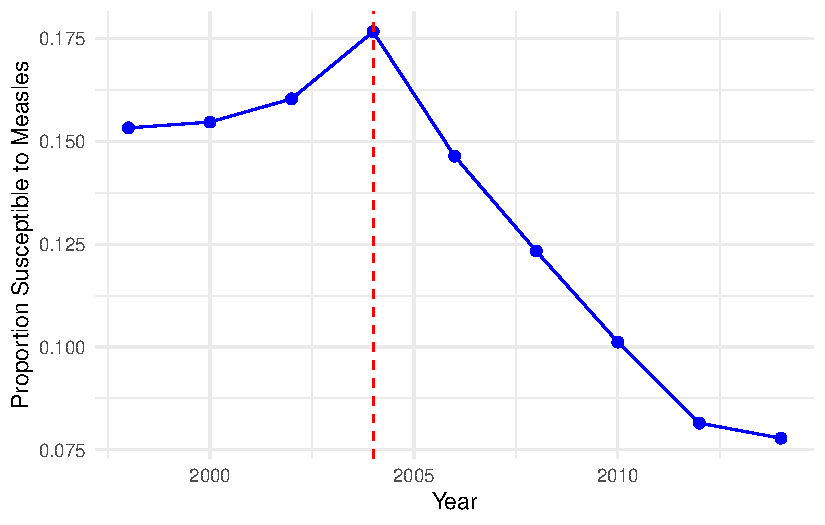
\includegraphics[width=0.8\textwidth,height=\textheight]{Group_14_Analysis_files/figure-pdf/fig-plot-1.pdf}

}

\caption{\label{fig-plot}Average Proprotion of Measle Susceptibility
against Year}

\end{figure}%

Figure~\ref{fig-plot} shows the proportion of the average measles
susceptibility across all IZ for each year, we can see a large decrease
in 2004 when the Wakefield article was retracted. After 2004 we see an
exponential decrease in the average proportion of measles susceptibility
untill out latest time point in 2014. 2004 had the largest value at
0.175 but we see this decrease each time period to eventually being just
above 0.075 in 2014.

\begin{figure}

\centering{

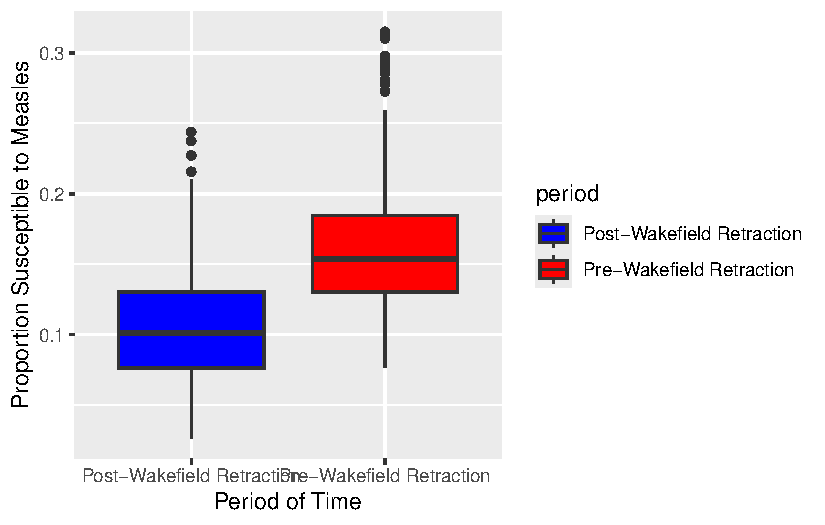
\includegraphics[width=0.8\textwidth,height=\textheight]{Group_14_Analysis_files/figure-pdf/fig-boxplot-1.pdf}

}

\caption{\label{fig-boxplot}Boxplots for average measle susceptibility
post and pre wakefield articlr retraction}

\end{figure}%

In Figure~\ref{fig-boxplot} we observe a clear change in average measles
susceptibility between the two groups. Following 2004, the median
susceptibility appears lower compared to the pre 2004 period, suggesting
a decrease after the retraction of the Wakefield article. Variability
appears similar between both groups whilst both groups appear to have
potential outliers, indiacting the presence of intermediate zones with
unusually high susceptibility.

\section{Formal Analysis}\label{formal-analysis}

To investigate whether the change in measles susceptibility occurred
specifically in 2004 alongside the retraction of the Wakefield article,
we fitted a grouped binomial logistic regression model. This approach is
appropriate because, for each intermediate zone and year, the data
record the number of susceptible pre-school children \emph{Y} out of the
total number of pre-school children \emph{N}. Therefore, the response is
naturally binomial. To answer this question, the model included an
overall time trend and a separate indicator for the year 2004. This
allowed us to assess whether measles susceptibility in 2004 deviated
from the general pattern observed over time.

Table~\ref{tbl-results} presents the estimated odds ratios from the
fitted model. The key parameter is the indicator for the year 2004,
since this directly tests whether 2004 represented a distinct change
point after accounting for the overall temporal trend in measles
susceptibility.

\begin{table}

\caption{\label{tbl-results}Results from the grouped binomial logistic
regression model}

\centering{

\fontsize{12.0pt}{14.0pt}\selectfont
\begin{tabular*}{\linewidth}{@{\extracolsep{\fill}}lrrrl}
\toprule
Term & Odds Ratio & Lower 95\% CI & Upper 95\% CI & p-value \\ 
\midrule\addlinespace[2.5pt]
(Intercept) & 0.207 & 0.200 & 0.214 & <0.001 \\ 
Time trend & 0.906 & 0.899 & 0.913 & <0.001 \\ 
Year 2004 indicator & 1.373 & 1.296 & 1.454 & <0.001 \\ 
\bottomrule
\end{tabular*}

}

\end{table}%

The coefficient for the 2004 indicator was positive and highly
statistically significant. The estimated odds ratio for the 2004 effect
was 1.373 (95\% CI: 1.296 to 1.454, 𝑝 \textless{} 0.001). This indicates
that, after accounting for the overall time trend, the odds of measles
susceptibility in 2004 were substantially higher than would be expected
from the broader temporal pattern alone. Therefore, the analysis
provides strong evidence that the change in measles susceptibility
occurred specifically in 2004, rather than being explained only by a
gradual trend over time.

The time trend was also statistically significant, with an estimated
odds ratio of 0.906 (95\% CI: 0.899 to 0.913, 𝑝 \textless{} 0.001). This
suggests that measles susceptibility generally declined over the study
period. However, despite this overall downward trend, the significant
positive 2004 effect indicates that 2004 represented a distinct
short-term increase in susceptibility.

\begin{figure}

\centering{

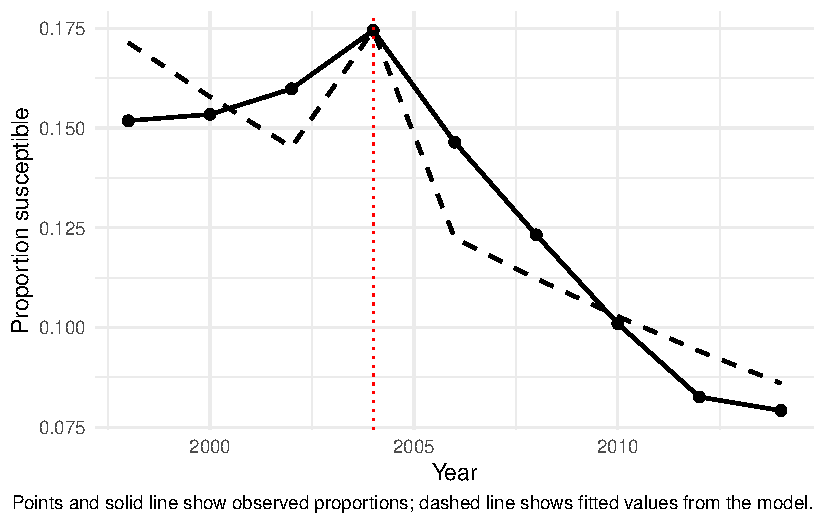
\includegraphics[width=0.8\textwidth,height=\textheight]{Group_14_Analysis_files/figure-pdf/fig-fitted-1.pdf}

}

\caption{\label{fig-fitted}Observed and fitted measles susceptibility by
year}

\end{figure}%

Figure~\ref{fig-fitted} compares the observed yearly proportions with
the fitted values from the model. The fitted values capture the overall
decline in measles susceptibility over time, while also indicating a
distinct upward deviation in 2004 relative to the long-term trend. This
visual pattern is consistent with the regression results and supports
the conclusion that 2004 was a distinct year in terms of measles
susceptibility.

Overall, there is strong statistical evidence that 2004 represented a
distinct deviation from the overall temporal trend. After accounting for
the general decline in measles susceptibility over time, the odds of
susceptibility in 2004 remained significantly higher than expected. This
suggests that the change in measles susceptibility occurred specifically
in 2004, consistent with the timing of the retraction of the Wakefield
article.

\section{Conclusions}\label{conclusions}

The exploratory analysis showed a noticeable difference between the
periods pre and post 2004, with lower average susceptibility observed
after 2004. The grouped binomial logistic regression model showed a
significant declining trend in measles susceptibility overtime. After
this trend, the indicator for year 2004 remained statistically
significant, with the odds ratio greater than 1. This indicates that
measles susceptibility in 2004 was higher than expected based on the
general trend.

Overall, the findings provide strong evidence that year 2004 represents
a clear deviation from the long term trend, indicating that the change
in susceptibility occurred specifically in that year rather than the
gradual decline. This pattern is consistent with the timing of the
retraction.

There's several limitations to this study: The analysis is observational
and cannot establish definite causality between the Wakefield article
retraction and the changes in susceptibility. The results should be
interpreted with caution. Other unmeasured factors (such as policy,
public health campaigns) may also have contributed to the observed
trend.

Future work could extend this analysis by incorporating additional
covariates, such as economic status and basic vaccination coverage, and
by applying more flexible models to better analyze potential trends and
effects.




\end{document}
